%%%%%%%%%%%%%%%%%%%%%%%%%%%%%%%%%%%%%%%%%
% Arsclassica Article
% LaTeX Template
% Version 1.1 (10/6/14)
%
% This template has been downloaded from:
% http://www.LaTeXTemplates.com
%
% Original author:
% Lorenzo Pantieri (http://www.lorenzopantieri.net) with extensive modifications by:
% Vel (vel@latextemplates.com)
%
% License:
% CC BY-NC-SA 3.0 (http://creativecommons.org/licenses/by-nc-sa/3.0/)
%
%%%%%%%%%%%%%%%%%%%%%%%%%%%%%%%%%%%%%%%%%

%----------------------------------------------------------------------------------------
%	PACKAGES AND OTHER DOCUMENT CONFIGURATIONS
%----------------------------------------------------------------------------------------

\documentclass[
10pt, % Main document font size
a4paper, % Paper type, use 'letterpaper' for US Letter paper
oneside, % One page layout (no page indentation)
%twoside, % Two page layout (page indentation for binding and different headers)
headinclude,footinclude, % Extra spacing for the header and footer
BCOR5mm, % Binding correction
]{scrartcl}
%%%%%%%%%%%%%%%%%%%%%%%%%%%%%%%%%%%%%%%%%
% Arsclassica Article
% Structure Specification File
%
% This file has been downloaded from:
% http://www.LaTeXTemplates.com
%
% Original author:
% Lorenzo Pantieri (http://www.lorenzopantieri.net) with extensive modifications by:
% Vel (vel@latextemplates.com)
%
% License:
% CC BY-NC-SA 3.0 (http://creativecommons.org/licenses/by-nc-sa/3.0/)
%
%%%%%%%%%%%%%%%%%%%%%%%%%%%%%%%%%%%%%%%%%

%----------------------------------------------------------------------------------------
%	REQUIRED PACKAGES
%----------------------------------------------------------------------------------------

\usepackage[
nochapters, % Turn off chapters since this is an article        
beramono, % Use the Bera Mono font for monospaced text (\texttt)
%eulermath,% Use the Euler font for mathematics
pdfspacing, % Makes use of pdftex’ letter spacing capabilities via the microtype package
dottedtoc % Dotted lines leading to the page numbers in the table of contents
]{classicthesis} % The layout is based on the Classic Thesis style

\usepackage{arsclassica} % Modifies the Classic Thesis package

\usepackage[T1]{fontenc} % Use 8-bit encoding that has 256 glyphs

\usepackage[utf8]{inputenc} % Required for including letters with accents

\usepackage{graphicx} % Required for including images
\graphicspath{{Figures/}} % Set the default folder for images

\usepackage{enumitem} % Required for manipulating the whitespace between and within lists

\usepackage{lipsum} % Used for inserting dummy 'Lorem ipsum' text into the template

%\usepackage{subfig} % Required for creating figures with multiple parts (subfigures)

\usepackage{amsmath,amssymb,amsthm} % For including math equations, theorems, symbols, etc

\usepackage{varioref} % More descriptive referencing

\usepackage{wrapfig}

\usepackage{caption}

\usepackage{subcaption}

%\usepackage[margin=0.5in]{geometry}

%----------------------------------------------------------------------------------------
%	THEOREM STYLES
%---------------------------------------------------------------------------------------

\theoremstyle{definition} % Define theorem styles here based on the definition style (used for definitions and examples)
\newtheorem{definition}{Definition}

\theoremstyle{plain} % Define theorem styles here based on the plain style (used for theorems, lemmas, propositions)
\newtheorem{theorem}{Theorem}

\theoremstyle{remark} % Define theorem styles here based on the remark style (used for remarks and notes)

%----------------------------------------------------------------------------------------
%	HYPERLINKS
%---------------------------------------------------------------------------------------

\hypersetup{
%draft, % Uncomment to remove all links (useful for printing in black and white)
colorlinks=true, breaklinks=true, bookmarks=true,bookmarksnumbered,
urlcolor=webbrown, linkcolor=RoyalBlue, citecolor=webgreen, % Link colors
pdftitle={}, % PDF title
pdfauthor={\textcopyright}, % PDF Author
pdfsubject={}, % PDF Subject
pdfkeywords={}, % PDF Keywords
pdfcreator={pdfLaTeX}, % PDF Creator
pdfproducer={LaTeX with hyperref and ClassicThesis} % PDF producer
}

 % Include the structure.tex file which specified the document structure and layout

%Proposition using definition counter
\newenvironment{proposition}[1][]{\refstepcounter{definition}\par\medskip
   \noindent \textbf{Proposition~\thedefinition. #1} \rmfamily}{\medskip}
 

\begin{document}

%----------------------------------------------------------------------------------------
%	TITLE AND AUTHOR(S)
%----------------------------------------------------------------------------------------

\title{\line(2,0){400}\\\normalfont\spacedlowsmallcaps{Reed-Muller Codes Achieve Capacity on Erasure Channels}\\\textit{\normalsize E2-207: Concentration Inequalities}\\\spacedlowsmallcaps{Course Project Report}
\footnote{Original work by \textit{S. Kudekar, S. Kumar, M. Mondelli, H. D. Pfister, E. \c{S}a\c{s}\u{o}glu and R. Urbanke.}}\\\line(1,0){400}} % The article title


\author{A report by \\ \\ \spacedlowsmallcaps{Ramakrishnan ,Soumya Subhra Banerjee}\\\spacedlowsmallcaps{Department of ECE,}\\ \spacedlowsmallcaps{Indian Institute of Science.}} % The article author(s) - author affiliations need to be specified in the AUTHOR AFFILIATIONS block

\date{\normalsize \today} % An optional date to appear under the author(s)

%----------------------------------------------------------------------------------------



%----------------------------------------------------------------------------------------
%	HEADERS
%----------------------------------------------------------------------------------------

\renewcommand{\sectionmark}[1]{\markright{\spacedlowsmallcaps{#1}}} % The header for all pages (oneside) or for even pages (twoside)
%\renewcommand{\subsectionmark}[1]{\markright{\thesubsection~#1}} % Uncomment when using the twoside option - this modifies the header on odd pages
\lehead{\mbox{\llap{\small\thepage\kern1em\color{halfgray} \vline}\color{halfgray}\hspace{0.5em}\rightmark\hfil}} % The header style

\pagestyle{scrheadings} % Enable the headers specified in this block
\newpage

%----------------------------------------------------------------------------------------
%	TABLE OF CONTENTS & LISTS OF FIGURES AND TABLES
%----------------------------------------------------------------------------------------

\maketitle % Print the title/author/date block


\setcounter{tocdepth}{2} % Set the depth of the table of contents to show sections and subsections only

\tableofcontents % Print the table of contents

%----------------------------------------------------------------------------------------
%	ABSTRACT
%----------------------------------------------------------------------------------------
\section*{abstract}
Efficiently decodable deterministic coding schemes which achieve channel capacity provably have been elusive until the advent of polar codes\cite{arikan} in the last decade.Further,the recent results by Urbanke et al.\cite{rm1} show that doubly transitive codes achieve capacity on erasure channel under MAP decoding.Urbanke and his group use threshold phenomenon observed in EXIT function , which capture the error probability ,to prove the same.These results were applied to Reed-Muller codes \cite{rm1}.Alternative proof of the fact Polar codes achieve capacity was suggested in \cite{vishva}.This report is a comprehensive study of threshold phenomenon in EXIT function and its applications as indicated above.

%----------------------------------------------------------------------------------------
%	INTRODUCTION
%----------------------------------------------------------------------------------------

\section{Introduction}
%----------Paper intro
The possibility of construction of low-complexity structured codes which provably achieve channel capacity ,having geometric structure and deterministic construction, have been explored since the conceptualization of channel capacity in ~\cite{shannon} . Turbo codes,LDPC ,spatially coupled LDPC were practical constructions towards this end.Polar codes~\cite{arikan} were the first provably capacity achieving codes for arbitrary Binary Input Symmetric Discrete Memoryless channels (BMS) with desirable complexity and deterministic structure.

Interestingly ~\cite{rm2},exploits the symmetry of deterministic linear codes, and threshold phenomenon in boolean function analysis to arrive at results summarized by the following theorem for transmission over a BEC channel.It is useful to point out that capacity of BEC($p$),$r=1-p$.

\textbf{Theorem - } A sequence of linear codes achieves capacity on
a memoryless erasure channel under MAP decoding if its blocklengths are strictly increasing, its code rates converge to some $r \in (0, 1)$, and the permutation group of each code is doubly transitive. 
The result, coupled with the fact that Reed-Muller are doubly transitive,extends to prove the capacity achieving nature of RM codes.It further provides an alternative prove of the same for Polar codes,without employing the inherent symmetry of the Hadamard matrix (consequently Arikan transform), from which polar codes derive their structure.

\subsection*{Brief introduction to Reed Muller codes:}
Reed-Muller codes are one of the oldest families of error correcting codes and use
concepts from algebra for the encoding and decoding process. The idea is to look
at the message as the coefficients of a multivariate polynomial of a suitable degree and pass 
its evaluations.They were introduced by Muller~\cite{muller} ,later Reed~\cite{reed} proposed a majority logic decoder for these codes. A binary Reed-Muller (RM) code with parameters $m$ and $v$ (the order) is a linear code of length $2^m$, dimension ${m \choose 0}+\ldots+{m \choose v}$ and minimum distance $2^{m-v}$. Although the possibility of RM codes achieving capacity under MAP decoding has been discussed in several papers, they being able to correct \emph{almost all} erasure patterns up to the capacity limit was not clear until this work.

\subsection*{Overall proof idea from the perspective of Threshold Phenomenon:}
\emph{Here we assume the reader has prior exposure to threshold phenomenon of boolean functions.}
\begin{figure}[h]
\centering 
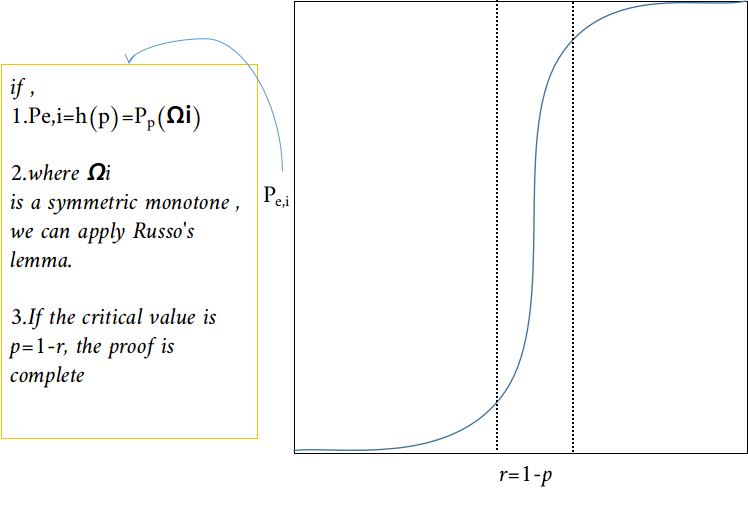
\includegraphics[width=0.75\columnwidth]{proofskeleton} 
\caption[]{"Achieving Capacity" from the perspective of threshold phenomenon. } % The text in the square bracket is the caption for the list of figures while the text in the curly brackets is the figure caption
\label{fig:proofskel} 
\end{figure}

For a sequence of binary linear codes with rate $r$ to be capacity achieving, the bit error probability,must converge to $0$ for any erasure rate below $1-r$.Towards this, (1)if the bit error probability under MAP-decoding can be captured by a function of erasure probability $(p)$,(2)which in turn is the measure of a symmetric monotone set ,then we shall observe threshold phenomenon,(3) if the threshold is sharp occuring at $p=1-r$ under the settings of stated theorem ,it provides a proof for the theorem.
Extrinsic information transfer (EXIT) function~\cite{exit} denoted by $h(p)$ in fig:\ref{fig:proofskel}, and the area theorem for EXIT functions~\cite{areathm} occupy a central role in this work. For a given input bit, the EXIT function is defined to be the conditional entropy of the input bit $i$ given the outputs associated with all other input bits.The value of the EXIT function at a particular erasure value is also directly related to the bit error probability under bit-MAP decoding,hence EXIT functions serve as (1).Furthermore, EXIT function can be associated with measure of set of erasure patterns $\Omega_i$ which are symmetric monotone sets for doubly transitive codes, solving(2).Finally application of area theorem solves (3).
The rest of the report elaborates on (1),(2) and (3) with focus on bit error probability under bit-MAP decoding.It extends the results to block error probability.

%----------------------------------------------------------------------------------------
%	PRELIMINARIES
%----------------------------------------------------------------------------------------

\section{Preliminaries}

Let $\mathcal{C}$ denote an $(N, K)$ proper binary linear code with length $N$ ,dimension $K$ ,minimum distance ($d_{min}$) atleast 2,and rate defined by $r \triangleq K/N$. We assume that a random codeword is chosen uniformly from this code and transmitted over a memoryless Binary Erasure Channel (BEC).A BEC with erasure probability $p$ is denoted by BEC($p$),or BEC($\underline{p}$) in case the erasure probability is different for each bit where $\underline{p} = (p_1 , \ldots , p_n)$ and
$p_i$ indicates the erasure probability for bit $i$.
The input and output alphabets of the BEC are denoted by $\mathcal{X} = \{0, 1\}$ and $\mathcal{Y} = \{0, 1, e\}$, respectively. Let $\underline{X} = (X_1 , \ldots , X_N) \in \mathcal{X}_N$ be a uniform random codeword and
$\underline{Y} = (Y_1 , \ldots, Y_N) \in \mathcal{Y}_N$ be the received sequence obtained by transmitting $\underline{X}$ through a BEC($p$).For a vector $a = (a_1 , a_2 , \ldots , a_N)$, the shorthand $\underline{a}_{\sim i}$ denotes
$(a_1 , \ldots , a_{i-1} , a_{i+1}, \ldots , a_N)$.
Let $\underline{a}$,$\underline{b}$ denote the indicator vectors of the sets $A \subseteq [N]$,$B \subseteq [N]$.We say that $A$ \emph{covers} $B$ if $B \subseteq A$, equivalently  $\underline{a}\leq\underline{b}$.For linear codes and erasure channels, it is possible to recover the transmitted codeword if and only if the erasure
pattern does not cover any codeword.Similarly,
it is possible to recover bit $i$ if and only if the erasure
pattern does not cover any codeword where bit $i$ is non-zero.


\subsection*{Bit and Block Erasure Probability} 
\paragraph*{Bit error probability:}Let $D_i : \mathcal{Y}^N \to \mathcal{X} \cup \{e\}$ denote the bit-MAP decoder for bit $i$ of $\mathcal{C}$. For a received sequence $\underline{Y}$ , if $X_i$ can be recovered uniquely, then $D_i(\underline{Y}) = X_i$. Otherwise, $D_i$ declares an erasure and returns $e$. Let the erasure probability for bit $i \in [N]$ be $$P_{b,i} \triangleq \mathbb{P}[D_i(\underline{Y}) \neq X_i].$$ and the average bit erasure probability be $$P_b \triangleq \frac{1}{N}\sum_{i=1}^N P_{b,i}.$$

Whenever bit $i$ can be recovered from a received sequence $\underline{Y}=\underline{y}$, $H(X_i | \underline{Y}=\underline{y}) = 0$. Otherwise, the uniform codeword assumption implies that the posterior marginal of bit $i$ given the observations is $\mathbb{P}(X_i = x|\underline{Y}=\underline{y}) = 1/2$ and $H(X_i |\underline{Y}=\underline{y}) = 1$. This immediately implies that $$P_{b,i} = H(X_i|\underline{Y})$$ and, $$P_b = \frac{1}{N}\sum_{i=1}^N  H(X_i|\underline{Y}).$$

\paragraph*{Block error probability:}TO BE EDITED BY RAMKI

\subsection*{MAP EXIT Functions} The vector EXIT function associated with bit $i$ of the (uniformly randomly chosen) codeword is $$h_i(\underline{p})\triangleq H(X_i | \underline{Y}_{\sim i}(\underline{p}_{\sim i})).$$ The average vector EXIT function is defined by $$h(\underline{p}) \triangleq \frac{1}{N}\sum_{i=1}^N h_i(\underline{p}).$$ Scalar EXIT functions are defined by choosing $\underline{p}=(p,p,\ldots,p)$.
\begin{align*}
H(X_i|\underline{Y}) &= \mathbb{P}(Y_i=e)H(X_i|\underline{Y}_{\sim i}, Y_i=e) + \mathbb{P}(X_i=Y_i)H(X_i|\underline{Y}_{\sim i}, Y_i=X_i)\\
&= \mathbb{P}(Y_i=e)H(X_i|\underline{Y}_{\sim i}).
\end{align*}
Therefore, $$P_{b,i}(p) = ph_i(p)$$ and $$P_b(p) = ph(p).$$
\begin{proposition}
The MAP EXIT function for the $i$th bit satisfies $h_i(p)=
\frac{\partial H(\underline{X}/\underline{Y}(\underline{p}))}{\partial p_i} $
\begin{proof}
\begin{align*}
H(\underline{X}/\underline{Y}(\underline{p})) &= H(X_i/\underline{Y}(\underline{p}))+H(X_{\sim i}/X_i,\underline{Y}(\underline{p})\\
&=H(X_i/\underline{Y}(\underline{p}))+H(X_{\sim i}/X_i,Y_{\sim i})  \text{ ,by memorylessness}\\
&=p_ih_i(p)+H(X_{\sim i}/X_i,Y_{\sim i}) 
\end{align*}
We note the second term is independent of $p_{i}$,the proposition follows on differentiation.
\end{proof}
\label{propn1}
\end{proposition}
\paragraph{Indirect Recovery} Consider a code $\mathcal{C}$ and the \emph{indirect recovery} of $X_i$ from the subvector $\underline{Y}_{\sim i}$ (i.e., the bit-MAP decoding of $Y_i$ from $\underline{Y}$ when $Y_i=e$). For $i \in [N]$, the set of erasure patterns that prevent indirect recovery of $X_i$ under bit-MAP decoding is given by 
\begin{definition}
$\Omega_i \triangleq \{A \subseteq [N]\backslash\{i\} : \exists B \subseteq [N]\backslash\{i\}, B \cup \{i\} \in \mathcal{C}, B \subseteq A\}$.
\label{defn2}
\end{definition}
For distinct $i,j \in [N]$, the set of erasure patterns where the $j$-th bit is \emph{pivotal} for the indirect recovery of $X_i$ is given by 
\begin{definition}
$\partial_j\Omega_i \triangleq \{A \subseteq [N]\backslash\{i\}: A\backslash \{j\} \notin \Omega_i, A \cup \{j\} \in \Omega_i \}$
\end{definition}
These are the erasure patterns where $X_i$ can be recovered from $\underline{Y}_{\sim i}$ if and only if $Y_j \neq e$.Note $\partial_j\Omega_i$ includes patterns from both $\Omega_i$ and $\Omega_i^c$.
\begin{proposition}
\label{propn4}
For a code $\mathcal{C}$ and transmission over a BEC, we have the following properties for the EXIT functions.
\begin{enumerate}
\item[(a)] The EXIT function associated with bit $i$ satisfies $$h_i(p) = \mu_{p}(\Omega_i)= \sum_{A \in \Omega_i} p^{|A|}(1-p)^{N-1-|A|}.$$
\item[(b)] For $j \in [N]\backslash\{i\}$, the partial derivative satisfies $$\frac{\partial h_i(\underline{p})}{\partial p_j}\Bigg|_{\underline{p}=(p,p,\ldots,p)} =\mu_{p}(\partial_j\Omega_i)= \sum_{A \in \partial_j\Omega_i} p^{|A|}(1-p)^{N-1-|A|}.$$
\item[(c)]The average EXIT function satisfies the \emph{area theorem} $$\int_0^1 h(p)dp = \frac{K}{N}.$$
\end{enumerate}
Where $\mu_{p}(\Omega)$ is the measure of the set of erasure patterns $\Omega$.
Here (a) and (b) follow from definition of conditional entropy and the fact that $H(X_i/\underline{Y}_{\sim i}=\underline{y}_{\sim i})=1$ when $A \cup \{i\}$ covers some codeword and decoding fails, and $0$ otherwise.(c) is a direct consequence of proposition \ref{propn1}
\end{proposition}
From the above discussion it is clear that the measure of the set $\Omega_i$ is equal to the probability of error for bit i , which in turn is equal to the ith EXIT function due to the uniform input assumption.

\subsection*{Permutations of linear codes} Let $S_N$ be the symmetric group on $N$ elements. The permutation group of a code is defined as the subgroup of $S_N$ whose group action on the bit ordering preserves the set of codewords.\\

\begin{definition}The permutation group $\mathcal{G}$ of a code $\mathcal{C}$ is defined to be $$\mathcal{G} = \{\pi \in S_N : \pi(A) \in \mathcal{C} \text{ for all } A \in \mathcal{C}\}.$$
\end{definition}

\begin{definition} - Suppose $\mathcal{G}$ is a permutation group. Then,
\begin{enumerate}
\item[(a)]$\mathcal{G}$ is \emph{transitive} if, for any $i,j \in [N]$, there exists a permutation $\pi \in \mathcal{G}$ such that $\pi(i)=j$, and
\item[(b)] $\mathcal{G}$ is \emph{doubly transitive} if, for any distinct $i,j,k \in [N]$, there exists a $\pi \in \mathcal{G}$ such that $\pi(i)=i$ and $\pi(j)=k$.
\end{enumerate}
\end{definition}

\begin{proposition}\emph{All EXIT functions are equal.}
Suppose the permutation group $\mathcal{G}$ of a code $\mathcal{C}$ is transitive. Then, for any $i \in [N]$, $$h(p) = h_i(p) \text{ for } 0 \le p\le 1.$$
\begin{proof}
claim:if $\mathcal{G}$ is transitive, then so is $\Omega_i$.
As $ A\in\Omega_i$,by definition\ref{defn2} $\exists B ,s.t.,B\cup\{i\} \in \mathcal{C}$, but by transitivity of $\mathcal{G}$, $\pi(B\cup\{i\}) \in \mathcal{C}$.Observe,$\pi(B\cup\{i\})=\pi(B)\cup\pi(\{i\})=\pi(B)\cup j$.Since $\pi(B) \subseteq \pi(A)$,it follows $\pi(A) \in \Omega_j$ .This indicates a bijection between $\Omega_i$ and $\Omega_j$,i.e,$|\Omega_i|=|\Omega_j|$.Moreover since, $ |A| =|\pi(A)|,$ propostion follows from proposition\ref{propn4} (a)
\end{proof}
\end{proposition}
\label{propn7}

\begin{proposition}
Suppose the permutation group $\mathcal{G}$ of a code $\mathcal{C}$ is doubly transitive. Then, for distinct $i,j,k \in [N]$, and any $0 \le p \le 1$, $$\frac{\partial h_i(\underline{p})}{\partial p_j'}\Bigg|_{\underline{p}=(p,p,\ldots,p)} = \frac{\partial h_i(\underline{p})}{\partial p_k'}\Bigg|_{\underline{p}=(p,p,\ldots,p)}.$$
\begin{proof}
Similar to the proof of proposition \ref{propn7}.Intuitively we expect that once we permute the locations , the bits which were pivotal must continue to remain so.Otherwise we could have decoded the concerned bit using simple permutations.
\end{proof}
\label{propn8}
\end{proposition}
\paragraph*{Summary of properties of EXIT function.}
\begin{description}
\item[1] $h_i(p)$ captures the bit error probability of MAP decoder.
\item[2] $h_i(p)$ is measure of $\Omega_i$.
\item[3] All EXIT functions are equal to average EXIT function h(p).
\item[4] $h_i(p)$ is strictly increasing and invertible.(follows from proposition \ref{propn4} (b))
\item[5] The area under the h vs p curve is the rate( by \emph{Area Theorem}).
\end{description}
We may notice here, that is $A\in\Omega_i$, it is a bit erasure pattern that causes error at position i, then $B\supset A$ will surely cause errors, and $B\in\Omega_i$.Thus $\Omega_i$ is monotone.Proving $\Omega_i $ is symmetric and has a sharp threshold at $p=1-r$, will establish that 2-transitive codes achieve Capacity.We will formalize this in the following subsections.

\subsection*{Capacity achieving codes and EXIT function}
\begin{definition}
Suppose $\{\mathcal{C}_n\}$ is a sequence of codes with rates $\{r_n\}$ where $r_n \to r$ for $r \in (0,1)$.
a) $\{\mathcal{C}_n\}$ is said to be \emph{capacity achieving} on the BEC under bit-MAP decoding, if for any $p \in [0, 1-r)$, the average bit-erasure probabilities satisfy $$\lim_{n \to \infty} P_b^{(n)}(p) = 0.$$
b) BLOCK MAP DECODING TO BE EDITED BY RAMKI
\end{definition}
\label{def10}

\begin{figure}[h]
\centering 
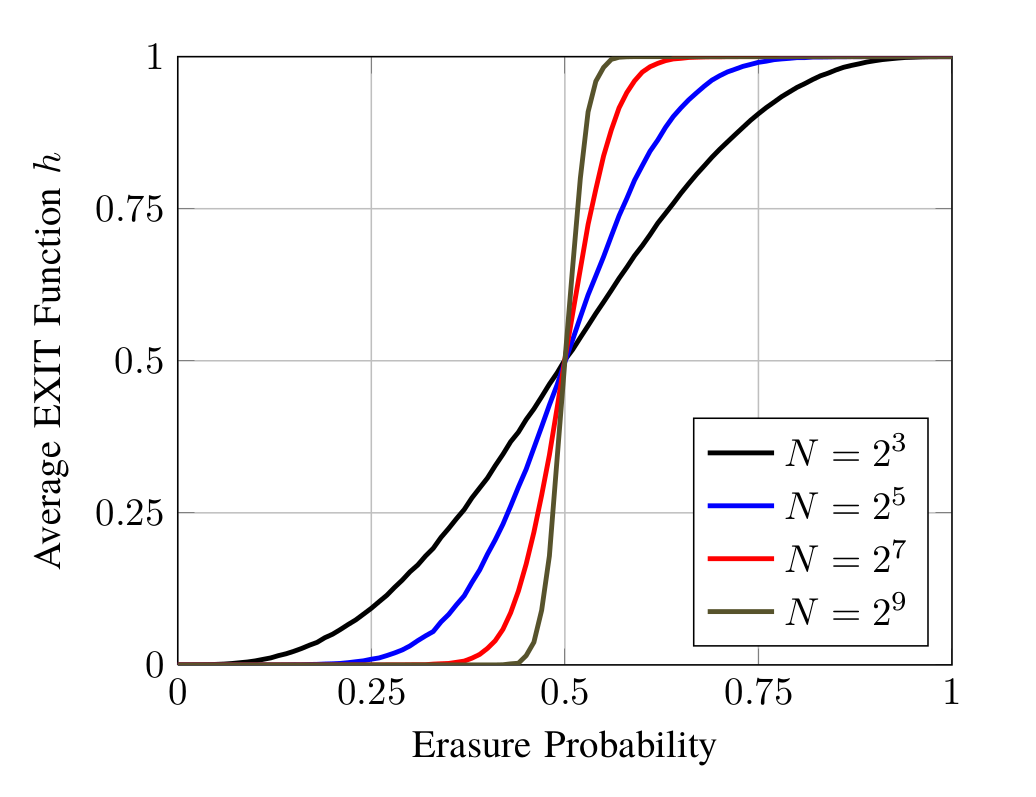
\includegraphics[width=0.75\columnwidth]{exitfun} 
\caption[]{The average EXIT function of the rate-$1/2$ Reed-Muller code with blocklength $N$.} % The text in the square bracket is the caption for the list of figures while the text in the curly brackets is the figure caption
\label{fig:exit} 
\end{figure}

The following theorem bridges capacity achieving codes, average EXIT functions, and the sharp transition framework that allows us to show that the transition width of certain functions goes to $0$. The average EXIT functions of some rate-$1/2$ Reed-Muller codes are shown in Figure~\ref{fig:exit}. Observe that as the blocklength increases, the transition width of the average EXIT function decreases. According to the following proposition, if this width converges to $0$, then Reed-Muller codes achieve capacity on the BEC under bit-MAP decoding.
\begin{proposition}
Let $\{\mathcal{C}_n\}$ be a seq. of codes with rates $\{r_n\}$, $r_n \to r$ for $r \in (0,1)$. The following are equivalent -
\begin{enumerate}
\item[S1:] $\{\mathcal{C}_n\}$ is capacity achieving on the BEC under bit-MAP decoding.
\item[S2:] The sequence of average EXIT functions satisfies
\[
    \lim_{n \to \infty} h^{(n)}(p)=\left\{
                \begin{array}{ll}
                  0 \text{ if } 0 \le p < 1-r\\
                  1 \text{ if } 1-r < p \le 1.\\
                \end{array}
              \right.
  \]
\item[S3:] For any $0 < \epsilon \le 1/2$, $$\lim_{n \to \infty} p_{1-\epsilon}^{(n)} - p_{\epsilon}^{(n)} = 0.$$
\end{enumerate}
\label{propn11}
\end{proposition}
\emph{where $h^{(n)}(p_{\epsilon}^{(n)})=\epsilon$.}\\
In short $S1\Rightarrow S2$, due to close relationship between bit error probability and average EXIT function pointed out in propostion \ref{propn4} .$S2\Rightarrow S3$,and $S3\Rightarrow S1$ by area theorem.Hence, proving S3 suffices to complete the proof.

\section{Main Result}
\subsection*{Doubly-transitive codes are Capacity Achieving under bit-MAP decoding. }
\begin{definition}
We can redefine $\Omega_i$ as a set of indicator vectors of $A$.Let,
\[
    [\phi_i(A)]_l=\left\{
                \begin{array}{ll}
                  \mathbf{1}_A(l) \text{ if } l < i\\
                  \mathbf{1}_A(l+1) \text{ if } l \ge i.\\
                \end{array}
              \right.
  \]
\begin{align*}
\Omega_i' &\triangleq \{\phi_i(A) \in \{0,1\}^{N-1} : A \in \Omega_i\}\\
\partial_j\Omega_i' &\triangleq \{\phi_i(A) \in \{0,1\}^{N-1}: A \in \partial_j\Omega_i\}.\\& =\{\underline{x} \in \{0,1\}^{N-1} | \mathbb{1}_{\Omega_i}(\underline{x}) \neq  \mathbb{1}_{\Omega_i}(\underline{x}^{(j)})\}
\end{align*}
\label{defn13}
\end{definition}
Here the last equality follows from definition of $\partial_j\Omega_i$.\\
Consider the space $\{0,1\}^M$ ,we can redefine measure $\mu_p$ such that $$\mu_p(\Omega) = \sum_{\underline{x} \in \Omega} p^{|\underline{x}|}(1-p)^{M-|\underline{x}|}, \text{ for }\Omega \subseteq \{0,1\}^M,$$ where the weight $|\underline{x}| = x_1 + x_2 + \ldots + x_M$ is the number of $1$'s in $\underline{x}$. 
\begin{definition}
For a monotone set $\Omega$.The influence of bit $j \in [N]$,is defined by,
$$I_j^{(p)}(\Omega)\triangleq \mu_p(\partial_j\Omega)$$
The total influence in defined by,
$$I^{(p)}\triangleq \sum^N_{j=1}I_j^{(p)}.$$
\label{defn15}
\end{definition}
Using proposition~\ref{propn4}(a) and proposition~\ref{propn7}, we have, 
$$h(p)=h_i(p)=\mu_p(\Omega_i')$$
Further,from proposition~\ref{propn4}(b), we get,
$$I_j^{p}(\Omega_i')=\mu_p(\partial_j\Omega_i') = \frac{\partial h_i(\underline{p})}{\partial p_j'}\Bigg|_{\underline{p}=(p,p,\ldots,p)}$$
where $j'$ is given by 
\[
    j'=\left\{
                \begin{array}{ll}
                  j \text{ if } j < i\\
                  j+1 \text{ if } j \ge i.\\
                \end{array}
              \right.
  \]
Since $\mathcal{G}$ is doubly transitive, from propostion~\ref{propn8}, $$I_j^{p}(\Omega_i') = I_k^{p}(\Omega_i') \text{ for all } j,k \in [N-1].$$
Hence,$\Omega_i$ is a \emph{symmetric monotone set.}

The following theorem could be seen as a consequence of the result by Talagrand~\cite{talagrand}.
\begin{theorem}
Let $\Omega$ be a monotone set and suppose that, for all $0 \le p \le 1$, the influences of all bits are equal $I_1^{(p)}(\Omega) = \ldots = I_M^{(p)}(\Omega)$. Then, for any $0 < \epsilon \le 1/2$, $$p_{1-\epsilon} - p_\epsilon \le \frac{2 \log \frac{1-\epsilon}{\epsilon}}{C\log (N-1)},$$ where $p_t = \inf\{p \in [0,1] : \mu_p (\Omega) \ge t\}$ is well defined because $\mu_p(\Omega)$ is strictly increasing in $p$ with $\mu_0(\Omega) = 0$ and $\mu_1(\Omega)=1$.
\label{thm19}
\end{theorem}
\begin{proof}
Using Russo's lemma~\cite{russo}.
\end{proof}
We see that $\Omega_i$ satisfies the conditions of Theorem~\ref{thm19}.
Hence,\\$$\lim_{n \to \infty} (p_{1-\epsilon} - p_\epsilon) = 0.$$
Further , using proposition~\ref{propn11}, we state,\\$\{\mathcal{C}_n\}$ is capacity achieving on the BEC under bit-MAP decoding.

\subsection*{Doubly-transitive codes are Capacity achieving under block-MAP decoding}
BLOCK ERROR TO BE EDITED BY RAMKI

\section*{APPLICATIONS}

\begin{theorem}
Let $\{\mathcal{C}_n\}$ be a sequence of codes where the blocklengths satisfy $N_n \to \infty$, the rates satisfy $r_n \to r$, and the permutation group $\mathcal{G}(n)$ (of $\mathcal{C}_n$) is doubly transitive for each $n$. If $r \in (0,1)$, then $\{\mathcal{C}_n\}$ is capacity achieving on the BEC under bit-MAP decoding.\\
In particular, $RM(v,m)$ codes achieve capacity.
\end{theorem}
\begin{proof}
Let the average EXIT function of $\mathcal{C}_n$ be $h^{(n)}$. Fix some $i \in [N]$. Since $\mathcal{G}$ is transitive, from Theorem~\ref{propn7}, $$h(p) = h_i(p) \text{ for all } p \in [0,1].$$

Consider the sets $\Omega_i'$ from Definitions~\ref{defn2} and~\ref{eqn8}, and let $M=N-1$. Observe that, from Theorem~\ref{propn4},
\begin{align*}
h_i(p) = \mu_p(\Omega_i'), &&I_j^{p}(\Omega_i') = \frac{\partial h_i(\underline{p})}{\partial p_j'}\Bigg|_{\underline{p}=(p,p,\ldots,p)}
\end{align*}
where $j'$ is given by 
\[
    j'=\left\{
                \begin{array}{ll}
                  j \text{ if } j < i\\
                  j+1 \text{ if } j \ge i.\\
                \end{array}
              \right.
  \]
Since $\mathcal{G}$ is doubly transitive, from Theorem~\ref{propn8}, $$I_j^{p}(\Omega_i') = I_k^{p}(\Omega_i') \text{ for all } j,k \in [N-1].$$

Using Theorem~\ref{thm16}, we have $$p_{1-\epsilon} - p_\epsilon \le \frac{2 \log \frac{1-\epsilon}{\epsilon}}{C\log (N-1)},$$ where $p_t$ is the functional inverse of $h$ as in Theorem~\ref{thm16}. Since $N \to \infty$ from the hypothesis, $$\lim_{n \to \infty} (p_{1-\epsilon} - p_\epsilon) = 0.$$

Now, using Theorem~\ref{propn10}, $\{\mathcal{C}_n\}$ is capacity achieving on the BEC under bit-MAP decoding.

Now, that $RM(v,m)$ codes achieve capacity follows from Theorem~\ref{rmdt}.
\end{proof}

\section{Conclusion}
\par This report is a summary of the result by S. Kudekar $et$ $al$~\cite{rm12} wherein it is proved that Reed Muller codes achieve capacity on erasure channels under bit-MAP decoding. The key ideas used in the proof could be enumerated as follows:
\begin{enumerate}
\item The permutation group of Reed Muller codes is doubly transitive.
\item For an erasure channel, the average EXIT function is directly related to the average bit erasure probability.
\item The average EXIT function satisfies the \emph{area theorem}. i.e., the area under the curve equals the rate of the code.
\item Showing that a sequence of codes is capacity achieving (the average bit erasure probabilities go to zero) is \emph{equivalent to} showing that the sharp transition width of EXIT functions go to zero.
\end{enumerate}
The interested reader may please see the original work ~\cite{rm1,rm2,rm12} for complete proofs and other details.


\newpage

%\begin{figure}[tb]
%\centering 
%\includegraphics[width=0.5\columnwidth]{GalleriaStampe} 
%\caption[An example of a floating figure]{An example of a floating figure (a reproduction from the \emph{Gallery of prints}, M.~Escher,\index{Escher, M.~C.} from \url{http://www.mcescher.com/}).} % The text in the square bracket is the caption for the list of figures while the text in the curly brackets is the figure caption
%\label{fig:gallery} 
%\end{figure}


%\begin{enumerate}[noitemsep] % [noitemsep] removes whitespace between the items for a compact look
%\item First item in a list
%\item Second item in a list
%\item Third item in a list
%\end{enumerate}

%------------------------------------------------


%----------------------------------------------------------------------------------------
%	RESULTS AND DISCUSSION
%----------------------------------------------------------------------------------------

%\section{Results and Discussion}
%
%\lipsum[10] % Dummy text
%
%%------------------------------------------------
%
%\subsection{Subsection}
%
%\lipsum[11] % Dummy text
%
%\subsubsection{Subsubsection}
%
%\lipsum[12] % Dummy text
%
%\begin{description}
%\item[Word] Definition
%\item[Concept] Explanation
%\item[Idea] Text
%\end{description}
%
%\lipsum[12] % Dummy text
%
%\begin{itemize}[noitemsep] % [noitemsep] removes whitespace between the items for a compact look
%\item First item in a list
%\item Second item in a list
%\item Third item in a list
%\end{itemize}
%
%\subsubsection{Table}
%
%\lipsum[13] % Dummy text
%
%\begin{table}[hbt]
%\caption{Table of Grades}
%\centering
%\begin{tabular}{llr}
%\toprule
%\multicolumn{2}{c}{Name} \\
%\cmidrule(r){1-2}
%First name & Last Name & Grade \\
%\midrule
%John & Doe & $7.5$ \\
%Richard & Miles & $2$ \\
%\bottomrule
%\end{tabular}
%\label{tab:label}
%\end{table}
%
%Reference to Table~\vref{tab:label}. % The \vref command specifies the location of the reference
%
%%------------------------------------------------
%
%\subsection{Figure Composed of Subfigures}
%
%Reference the figure composed of multiple subfigures as Figure~\vref{fig:esempio}. Reference one of the subfigures as Figure~\vref{fig:ipsum}. % The \vref command specifies the location of the reference


%----------------------------------------------------------------------------------------
%	BIBLIOGRAPHY
%----------------------------------------------------------------------------------------

\renewcommand{\refname}{\spacedlowsmallcaps{References}} % For modifying the bibliography heading

\bibliographystyle{unsrt}

\bibliography{sample.bib} % The file containing the bibliography

%----------------------------------------------------------------------------------------

\end{document}